\section*{Graphs, vertices, and edges%
\TAGS{graph}}

A \emph{graph} $G$ is a set of vertices $V$ and a set of edges $E$,
where each edge is a pair of vertices.
\begin{center}
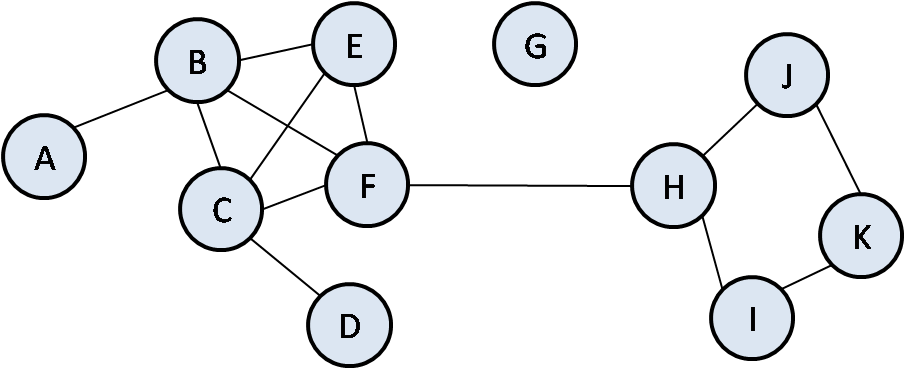
\includegraphics[width=0.50\textwidth]{\img/graph.png}
\end{center}
For example, the graph above would be described by giving the vertex
set and the edge set as in
$$
\begin{array}{lcl@{}}
   V &=& \{A,B,C,D,E,F,G,H,I,J,K\}
\\ E &=& \{(A,B),(B,C),(B,E),(B,F),(C,D),(C,E),(C,F),(E,F),(F,H),(H,I),(H,J),(I,K),(J,K)\}
\end{array}
$$
(For brevity, only edges in one direction are listed. This is okay because the
graph above is \emph{undirected}.)

The \emph{subgraph} consisting of only vertices $B$, $C$, $E$, and
$F$ is called a \emph{complete graph} because an edge exists between
every two of those vertices.


\checkpoint*{\TAGS{graph}}

Let $T(n)$ be the number of edges in a complete graph with $n$
vertices. Write a recursive formula for $T(n)$. You will need to write
two expressions --- one for the base case and one for the recursive
case.

\begin{solution}
$$
\left\{
\begin{array}{lll}
   T(1) &=& 0
\\ T(n) &=& n-1 + T(n-1)
\end{array}
\right.
$$
A graph with $1$ vertex cannot have any edges. You can enumerate the edges in a
graph with $n$ vertices by choosing a vertex and partitioning the edges by
whether they are connected to that vertex. There are $n-1$ connected to that
vertex, and all the rest form a complete graph with the other $n-1$ vertices.
\end{solution}


\checkpoint*{\TAGS{graph-representation}}

Recall from lecture that we discussed two ways of representing graphs:
adjacency matrices and adjacency lists. Draw the adjacency matrix and the
adjacency list for the graph above.

\vfill
\begin{solution}

Adjacency Matrix:
\begin{verbatim}
  | A B C D E F G H I J K
-------------------------
A | 0 1 0 0 0 0 0 0 0 0 0
B | 1 0 1 0 1 1 0 0 0 0 0
C | 0 1 0 1 1 1 0 0 0 0 0
D | 0 0 1 0 0 0 0 0 0 0 0
E | 0 1 1 0 0 1 0 0 0 0 0
F | 0 1 1 0 1 0 0 1 0 0 0
G | 0 0 0 0 0 0 0 0 0 0 0
H | 0 0 0 0 0 1 0 0 1 1 0
I | 0 0 0 0 0 0 0 1 0 0 1
J | 0 0 0 0 0 0 0 1 0 0 1
K | 0 0 0 0 0 0 0 0 1 1 0
\end{verbatim}

Adjacency List:
\begin{verbatim}
A | B
B | A, C, E, F
C | B, D, E, F
D | C
E | B, C, F
F | B, C, E, H
G |
H | F, I, J
I | H, K
J | H, K
K | I, J
\end{verbatim}
\end{solution}


\checkpoint*{\TAGS{complexity, graph-representation}}

In terms of $|V|$ and $|E|$, give a big-O bound for the
\lstinline'graph_hasedge' operation for both the adjacency matrix and
adjacency list representations.

\begin{solution}
\begin{description}
\item[Adjacency Matrix: ]%
  $O(1)$, because this requires two array accesses.
\item[Adjacency List: ]%
  $O(|V|)$, because this requires an array access followed by a search
  through the neighbors (bounded by $|V|$). Can also be $O(min(|V|, |E|))$
  if you want to be precise.
\end{description}
\end{solution}


\checkpoint*{\TAGS{graph, graph-representation}}

We call a graph \emph{sparse} if it has relatively few edges and
\emph{dense} if it has relatively many edges. Which representation
might you want to use for a sparse graph? What about for a dense
graph? Why?

\begin{solution}
\begin{description}
\item[Sparse graph: ]%
  Since there are so few edges, an adjacency list will work well
  because each list will be short, and it saves memory in comparison
  to an adjacency matrix.
\item[Dense graph: ]%
  Since there are so many edges, an adjacency matrix can efficiently
  store the edge information and will allow edge lookup in $O(1)$.
\end{description}
\end{solution}
